\chapter{Introduction}
\section{Background}
%%%%%%%%%
% Cloud %
%%%%%%%%%


%%%%%%%%%%%%%%%%%%%%
% Virtual Machines %
%%%%%%%%%%%%%%%%%%%%


%%%%%%%%%%%%%%
% Containers %
%%%%%%%%%%%%%%


%%%%%%
% CI %
%%%%%%


\section{Aims}
This paper aims to study how different container orchestrated OCI build-tools compare to each other. The build-tools in table \ref{tab:build_tools} will be compared with the aspects in table \ref{tab:aspects}. The build-tools were chosen by communicating with Omegapoint and by reading multiple sources \cite{build_compare} \cite{jib}.

\section{Objectives}

\section{Risk Register}
\begin{sidewaysfigure}[h!]
    \centering
    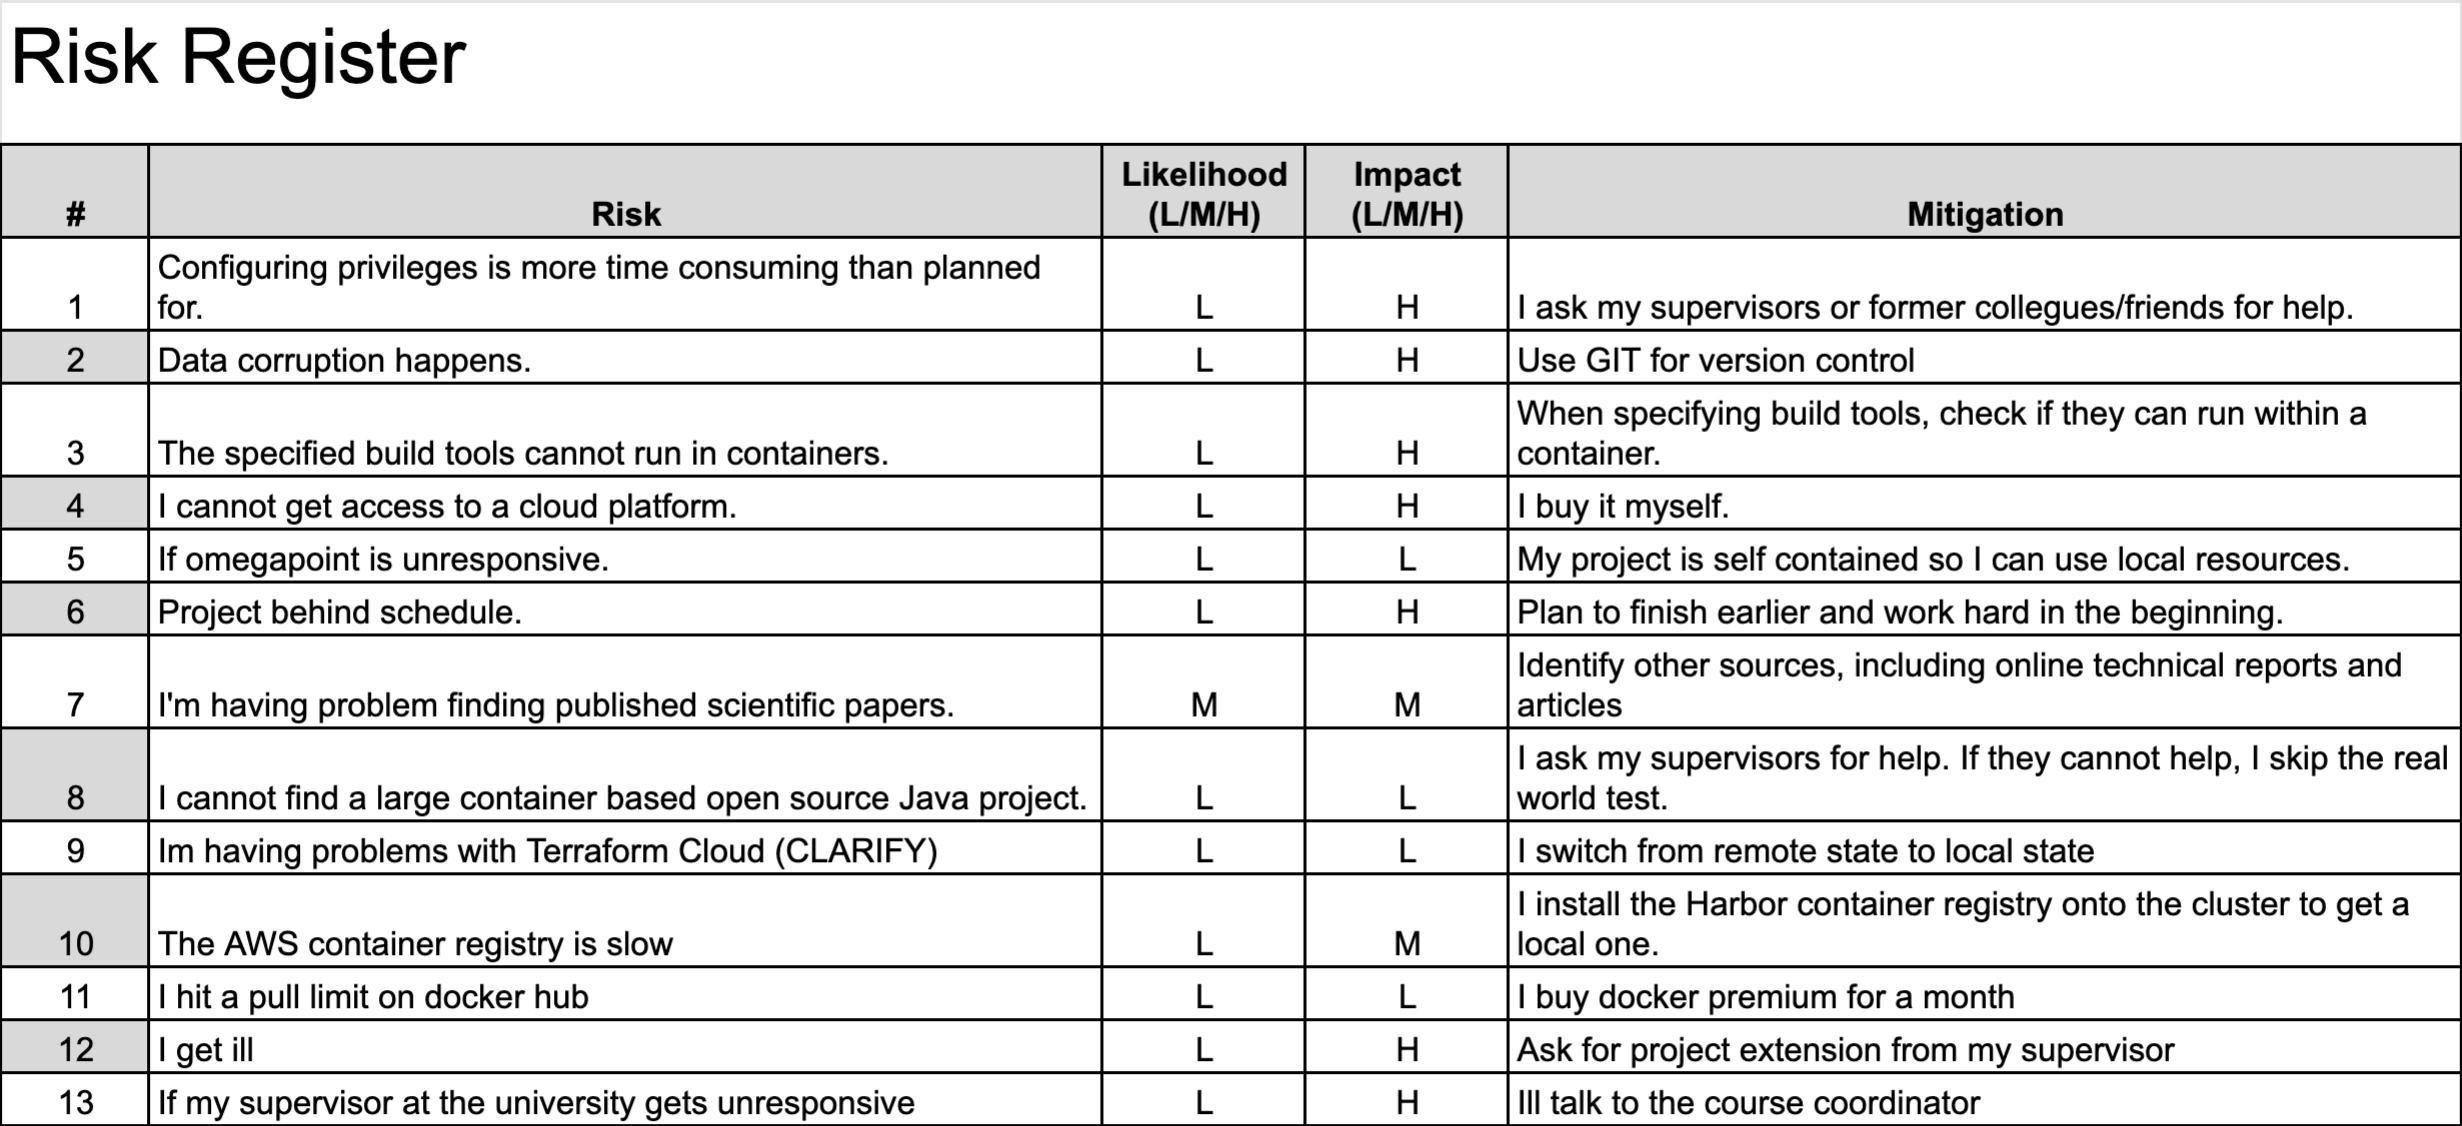
\includegraphics[width=\linewidth]{risks.png}
    \caption{Risk register}
    \label{fig:risk_register}
\end{sidewaysfigure}

\section{Gantt Chart}
\begin{sidewaysfigure}[h!]
    \centering
    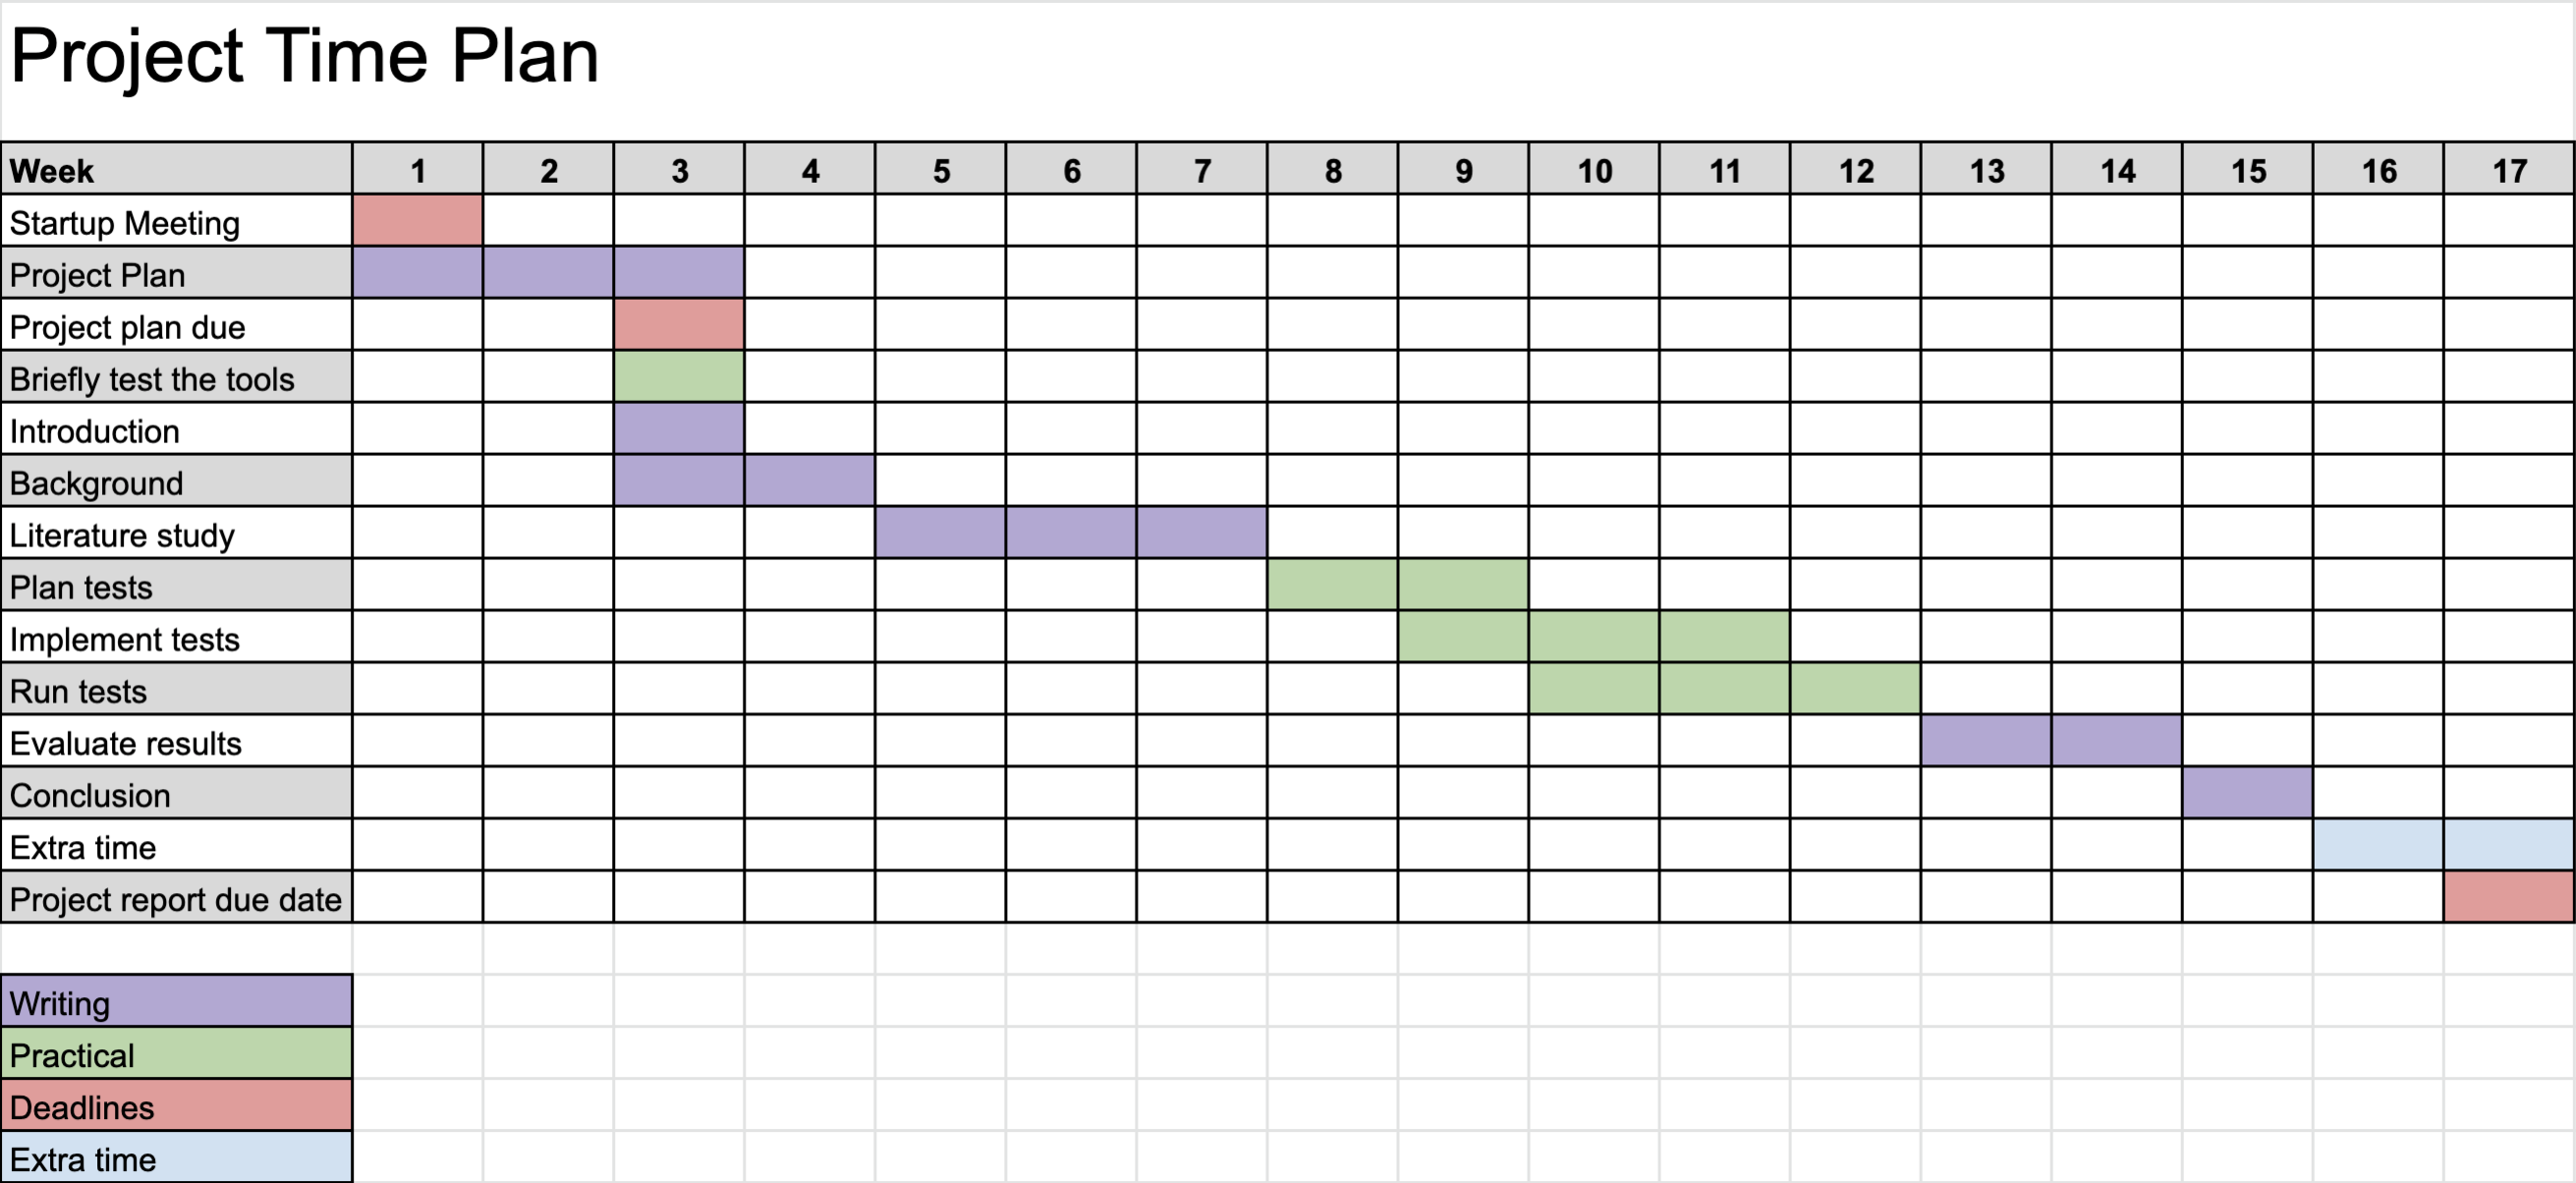
\includegraphics[width=\linewidth]{gantt.png}
    \caption{Project time plan in the form of a Gantt chart}
    \label{fig:gantt}
\end{sidewaysfigure}

%\def\cloudperks{\footnote{Salesforce UK. What are the Advantages of Cloud Computing? 10 Reasons to Move to the Cloud. Read 2021-01-18. \url{https://www.salesforce.com/uk/blog/2015/11/why-move-to-the-cloud-10-benefits-of-cloud-computing.html}}}
%\def\cloudhistory{\footnote{IBM Cloud Team. IBM. A Brief History of Cloud Computing. Read 2021-01-18. \url{https://www.ibm.com/cloud/blog/cloud-computing-history}}}
%\def\rhcontainers{\footnote{Red Hat. What's a Linux container?. Read 2021-01-18. \url{https://www.redhat.com/en/topics/containers/whats-a-linux-container}}}
%\def\ocicontainers{\footnote{OCI. About the Open Container Initiative. Read 2021-01-18. \url{https://opencontainers.org/about/overview/}}}
%\def\whatkubernetes{\footnote{Kubernetes. What is Kubernetes?. Read 2021-01-18. \url{https://kubernetes.io/docs/concepts/overview/what-is-kubernetes/}}}
%
%\chapter{Introduction}
%When computing was new, all computations were local. Today, computations are done remotely. The cloud allows companies of all sizes to use resilient and highly available solutions\cloudperks. Different cloud providers usually provide similar features and user experiences. Therefore, it is possible to use the right platform for the right job. Cloud services provide easily accessible virtual machines. which are scriptable and easily configurable to make software deployment easier. Virtual Machines provide easy startup, accessibility and backup management. However, they are stateful, making them almost as hard as their predecessor, bare-metal machines, to manage if scaled. Virtual machines also have a noticeable performance overhead since their host operating system has to emulate the hardware and run an entire operating system around all applications.
%
%To solve these problem stateless containers were developed. Containers function by sharing their kernel with the host machine and only running the most necessary software\rhcontainers. Containers also make it possible to run reproducible code and allows the tested software (and its dependencies) to be used in production. One of the most popular types of containers is OCI\ocicontainers (Open Container Initiative) containers. It is a specification of stateless Linux containers that states their interface; this allows the development of multiple runtimes and build-tools. A container orchestrator is often used to connect containers running on different machines to each other. They have dramatically simplified the deployment and scaling of distributed software. The most common orchestrator is called Kubernetes\whatkubernetes and allows a cluster of machines, from a users perspective, to function as a single entity. Kubernetes is also easily extended with custom software like logging, security scanning and backups.  
%
%A common approach when developing software is Continuous Integration (CI) and Continuous Deployment (CD). It is a workflow which runs pipelines on each commit to a VCS for automatic testing, linting and more. It allows for seamless integration of tested code into a repository and then automatically deploying it to production. In these pipelines, containers are often built and pushed to a registry. There exists a lot of different container build-tools which has different advantages and disadvantages. It is often desirable to run pipelines within Kubernetes to make use of its great ecosystem. However, container build-tools are often supposed to run directly on an operating system. That is sub-optimal in a Kubernetes environment due to its insecure nature when allowing access to the host node. 
%
%\section{Aim}
%This paper aims to study how different container orchestrated OCI build-tools compare to each other. The build-tools in table \ref{tab:build_tools} will be compared with the aspects in table \ref{tab:aspects}. The build-tools were chosen by communicating with Omegapoint and by reading multiple sources \cite{build_compare} \cite{jib}.
%
%% build an evaluation framework for measureing the effectiveness of oci build-tools.
%
%% objectives
%% what are the most appropriate metrics to compare oci build tools
%% what are the different environments? security?
%% can i create a recommendation system?
%
%\begin{table}[h!]
%    \centering
%    \begin{tabular}{l|l}
%        \textbf{Build tool} & \textbf{Version} \\
%        \hline
%        Kaniko & 1.3.0 \\
%        \hline
%        Buildah & 1.19.2 \\
%        \hline
%        Img & 0.5.11 \\
%        \hline
%        BuildKit & 0.8.1 \\
%        \hline
%        Google Jib & 0.17.0
%    \end{tabular}
%    \caption{Build-tools}
%    \label{tab:build_tools}
%\end{table}
%
%\begin{table}[h!]
%    \centering
%    \begin{tabular}{l|l}
%        \textbf{Aspect} & \textbf{Description} \\
%        \hline
%        Security & What are the known security issues?\\
%        \hline
%        Performance & How performant are the different build-tools?\\
%        \hline
%        Cache & How efficient are the build-tools at handling cache?\\
%        \hline
%        Usability & How good is the user experience of the build tool?\\
%        \hline
%        Basic Features & Are all expected basic features supported?\\
%        \hline
%        Cost & What is the cost of using the build tool? \\
%    \end{tabular}
%    \caption{Comparison aspects}
%    \label{tab:aspects}
%\end{table}
%
%\section{Earlier Work and study}
%To better understand the field, earlier research will be studied. It is done to lay a basis for the project and better strengthen the decisions made when developing and performing the tests. Much of the scientific work done in the cloud field is not published in scientific journals but on company pages. Therefore scientific papers, papers from large companies and papers written by experts on the subjects will be read and utilized. The examined subjects will be:
%
%\begin{enumerate}
%    \item Cloud
%    \item OCI Containers
%    \item Container security
%    \item CI/CD Pipelines
%    \item Kubernetes
%\end{enumerate}
%
%\section{Mentorship}
%Paul Townend at Umeå University will be the mentor for this project. We will have a meeting every week and continuously communicate with email. The master thesis is written with the help of the company Omegapoint, and we will use Slack for internal communication and have a meeting as often as we desire. 
%
%\begin{table}[h!]
%    \centering
%    \begin{tabular}{l|l|l}
%        \textbf{Mentor} & \textbf{Name} & \textbf{Email} \\
%        \hline
%        University & Paul townend & \href{mailto:paul.townend@umu.se}{paul.townend@umu.se} \\
%        \hline
%        Omegapoint & Mattias Persson & \href{mailto:mattias.persson@omegapoint.se}{mattias.persson@omegapoint.se} \\
%                   & Anders Sigfridsson & \href{mailto:anders.sigfridsson@omegapoint.se}{anders.sigfridsson@omegapoint.se} \\    
%    \end{tabular}
%    \caption{Mentors and contact information}
%    \label{tab:mentors}
%\end{table}
%
%\section{Risk Register}
%\begin{sidewaysfigure}[h!]
%    \centering
%    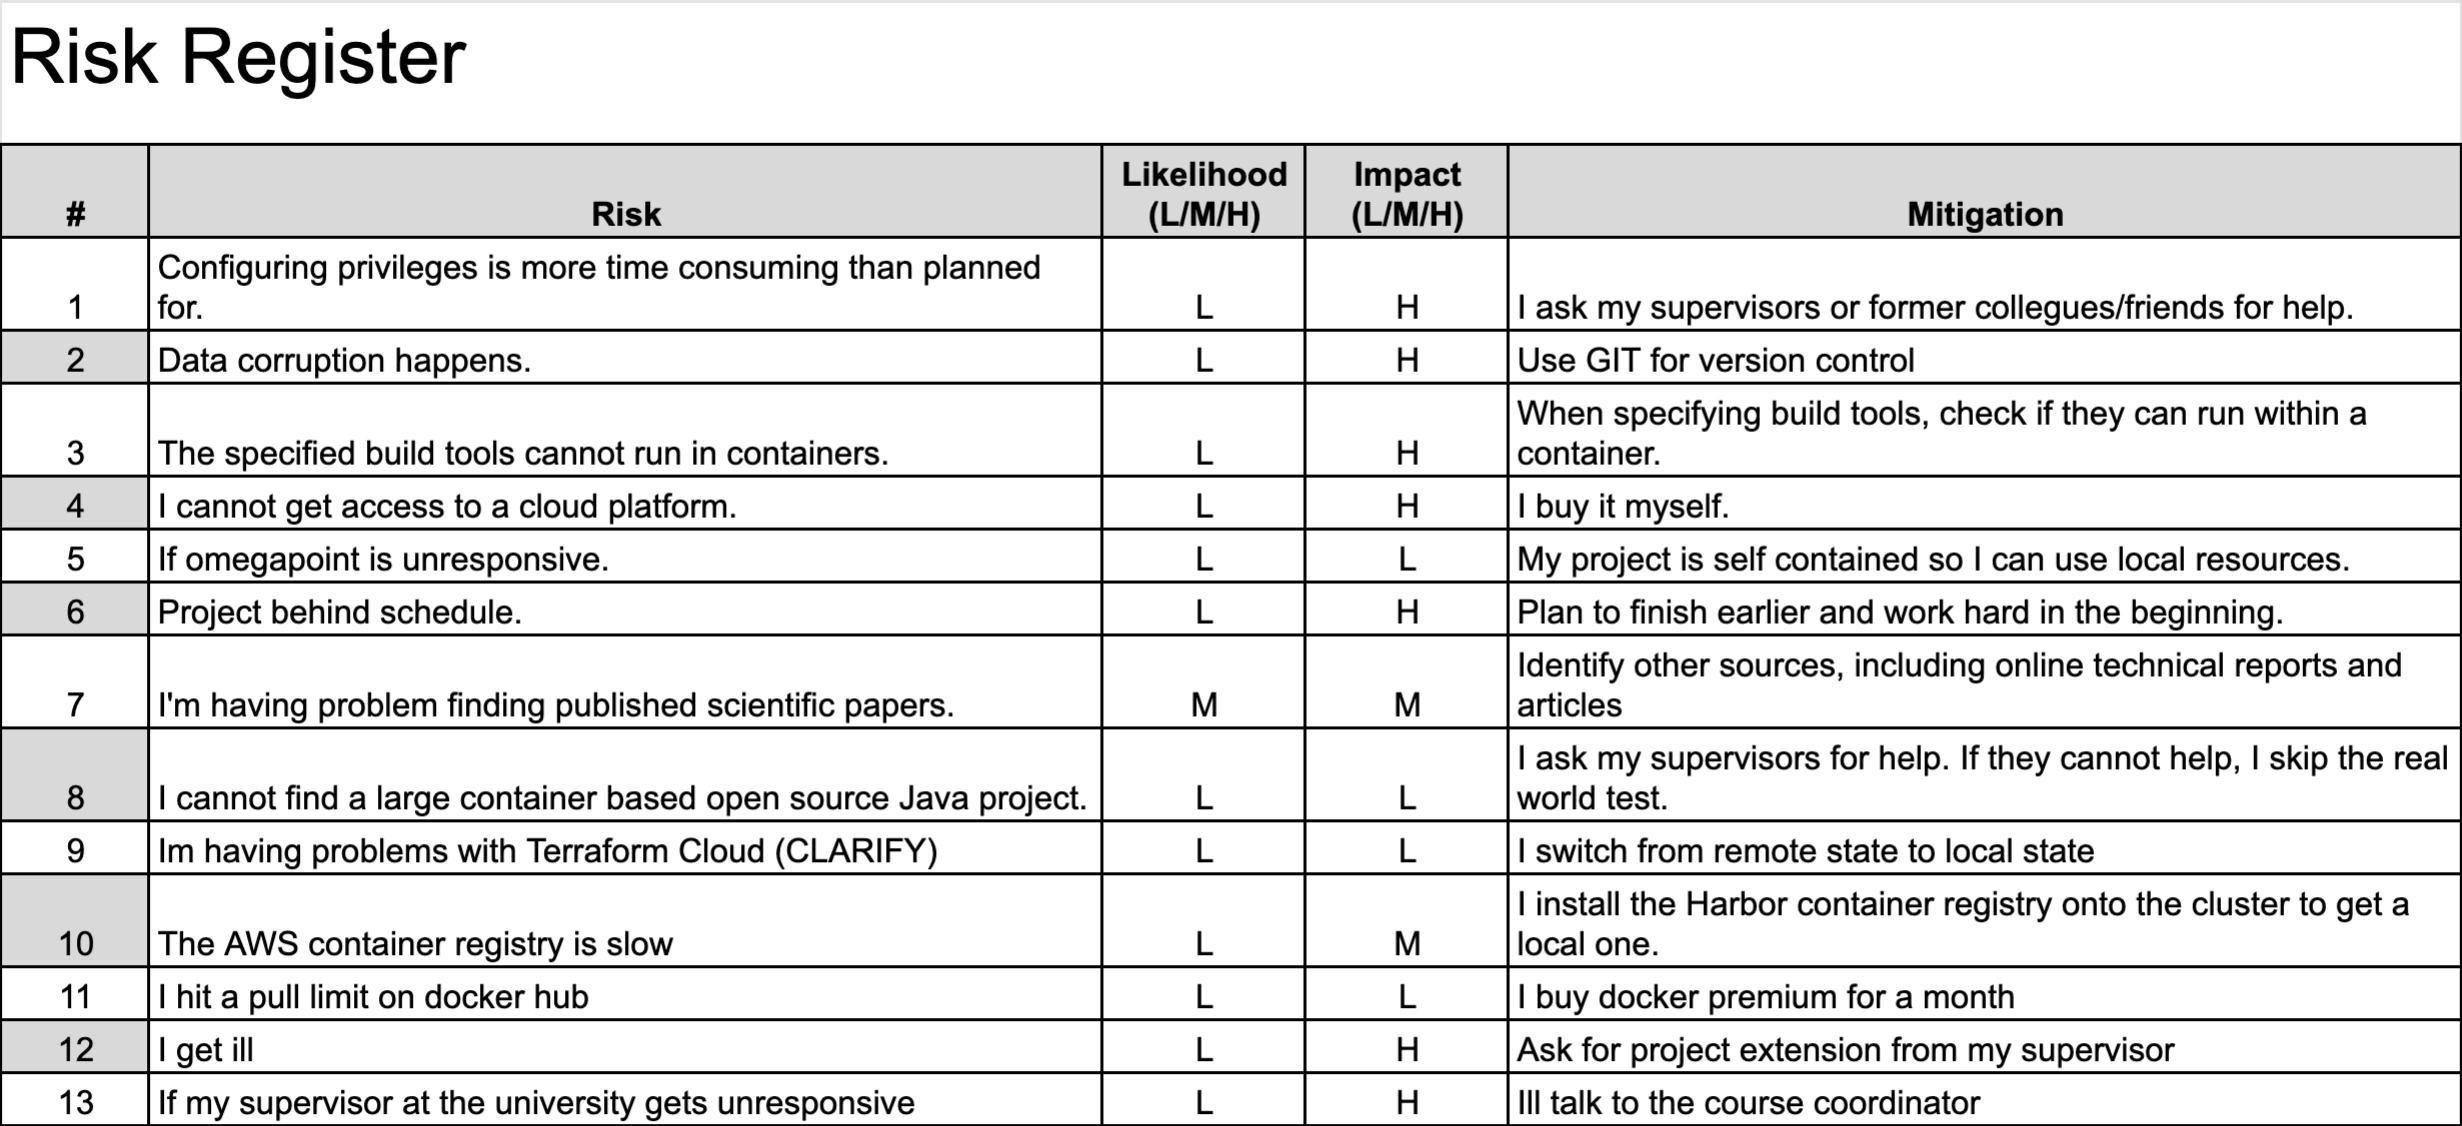
\includegraphics[width=\linewidth]{risks.png}
%    \caption{Risk register}
%    \label{fig:risk_register}
%\end{sidewaysfigure}
%
%\section{Gantt Chart}
%\begin{sidewaysfigure}[h!]
%    \centering
%    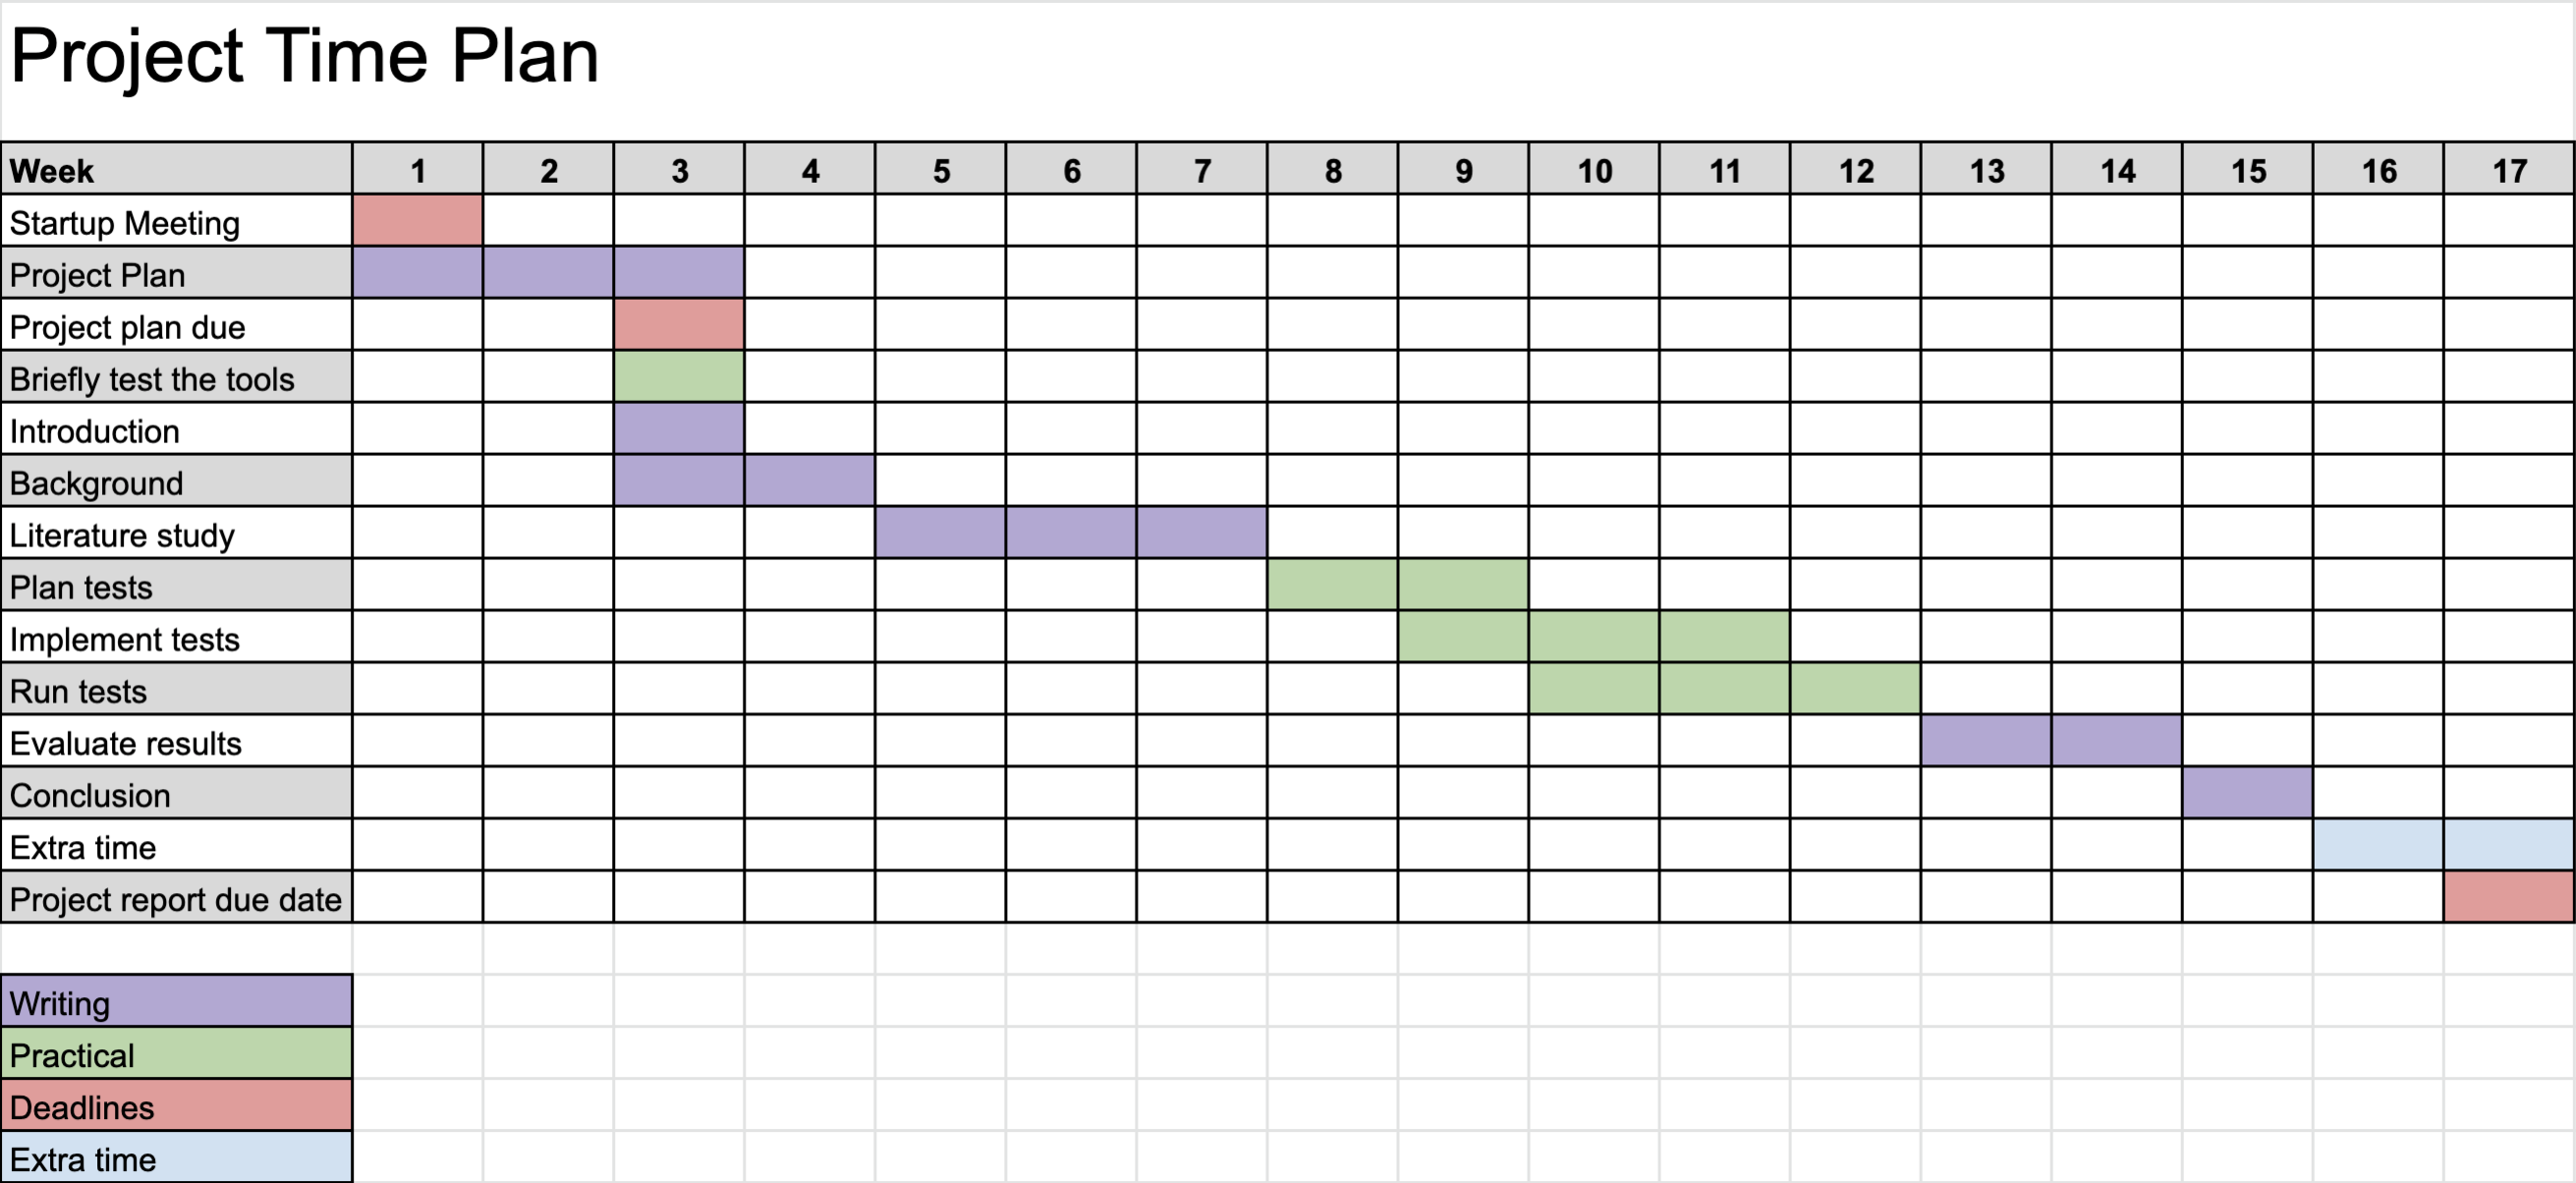
\includegraphics[width=\linewidth]{gantt.png}
%    \caption{Project time plan in the form of a Gantt chart}
%    \label{fig:gantt}
%\end{sidewaysfigure}